\chapter{Real-Time Operating Systems}
\label{cha:rtos}

This project has been developed and tested on bare-metal applications to ensure
its correctness in simple environments. However, many embedded devices are
designed to accomplish more complex tasks and they need special environments to
support the execution. The purpose of this chapter is to provide insights on how
the project could be implemented to work with Real-Time Operating Systems (RTOS)
to secure and support complex tasks and environments. Specifically, we provide an
implementation idea for two famous RTOSes, \textit{Free Real-Time Operating
System} (\textit{FreeRTOS}) and \textit{Zephyr RTOS}, depicting their strengths
and the limitations that may arise during implementation.

\section{FreeRTOS}
\label{sec:rtos_rtos}

\textit{FreeRTOS}\cite{freertos} is an open-source, lightweight, Real-Time Operating
System kernel designed for embedded systems. In recent years, \textit{FreeRTOS}
has become one of the most widely used \textit{RTOS} kernels in embedded applications,
particularly in microcontrollers, because of its simplicity, efficiency, scalability,
and portability. \textit{FreeRTOS} is mostly used in applications that require
reliable, deterministic behavior in resource-constrained environments such as medical
devices, IoT devices, and automotive systems.

\textit{FreeRTOS} provides many key features:
\begin{itemize}
  \item Real-Time Scheduling: \textit{FreeRTOS} supports real-time scheduling with
    both preemptive and cooperative multitasking. In preemptive scheduling, tasks
    are prioritized and can interrupt lower-priority tasks, while in cooperative
    multitasking, tasks yield control to others explicitly. Moreover, it uses priority-based
    scheduling, allowing developers to assign priority levels to tasks based on
    their timing requirements;

  \item Task Management: Tasks in \textit{FreeRTOS} are individual threads of execution,
    each with its stack and context. The kernel allows the creation, deletion, and
    management of tasks dynamically. Each task operates in its own context, which
    the kernel saves and restores during context switching;

  \item Memory Management: \textit{FreeRTOS} provides several memory allocation schemes,
    including static and dynamic allocation, through its portable memory allocation
    subsystem. It supports different heap management schemes (\textit{heap\_1}
    through \textit{heap\_5}), offering varying levels of complexity and memory usage
    optimization. These schemes allow developers to balance between simplicity
    and flexibility;

  \item Interrupt Handling: \textit{FreeRTOS} is designed to work seamlessly with
    hardware interrupts, allowing Interrupt Service Routines (ISR) to
    communicate with tasks through mechanisms like queues and semaphores. The kernel
    offers a low-latency method for ISR handling, enabling efficient
    communication between ISRs and tasks while ensuring minimal delay in task
    scheduling;

  \item Software Timers: \textit{FreeRTOS} includes a timer API, allowing
    developers to create software timers that automatically trigger callback
    functions after a specified period. This feature helps to manage time-dependent
    operations without creating dedicated tasks;

  \item Portability and Scalability: \textit{FreeRTOS} is highly portable and can
    be adapted to run on numerous processor architectures, including \textit{ARM
    Cortex-M}, \textit{ARM Cortex-A}, \textit{RISC-V}, and various other
    architectures. It is structured in a way that allows developers to scale applications
    easily by adding or removing tasks, memory management schemes, and communication
    mechanisms as needed;

  \item Debugging and Traceability: \textit{FreeRTOS} provides support for debugging
    and traceability, offering hooks that allow users to gather runtime
    statistics and monitor task execution patterns.
\end{itemize}

With all these features it is easy to see why \textit{FreeRTOS} has become a standard
in the community. However, \textit{FreeRTOS} presents some limitations like the
limited built-in security and the lack of support for multicore processing. Some
of these flaws have been addressed by community users and companies with alternative
versions of the Operating System. For example, \textit{Espressif} presented
\textit{IDF FreeRTOS}\cite{idfrtos}, a version of \textit{FreeRTOS} which
provides support for multicore processing. Moreover, \textit{highintegritysystems}
developed \textit{SAFERTOS}\cite{safertos}, a redesign of the \textit{FreeRTOS} kernel
to enhance security.

Overall, \textit{FreeRTOS} is a powerful choice for developers working with embedded
systems that require real-time capabilities, low overhead, and efficient resource
management. Its design balances simplicity with flexibility, making it suitable for
a wide variety of applications from small IoT devices to more complex industrial
systems.

\section{Zephyr RTOS}
\label{sec:rtos_zephyr}

\textit{Zephyr RTOS}\cite{zephyrtos} is an open-source, Real-Time Operating System
designed for embedded systems and IoT applications. Developed under the Linux
Foundation, it offers a lightweight, modular, and scalable platform that supports
a wide range of devices, from simple microcontrollers to complex systems. Widely
adopted across IoT devices, industrial automation, medical equipment, and
automotive systems, \textit{Zephyr RTOS} excels in environments requiring
reliability, efficiency, and resource optimization.

A key feature of \textit{Zephyr} is its scalability and modularity. Its
architecture enables developers to include only the features they need, optimizing
memory usage and performance for resource-constrained devices. The kernel
supports multiple configurations, making it adaptable for both simple single-threaded
tasks and advanced multi-threaded applications. Additionally, \textit{Zephyr} is
designed to deliver deterministic, time-critical performance, ensuring minimal
latency and high reliability.

\textit{Zephyr} includes advanced security features such as memory protection,
secure boot, and support for Hardware Security Modules (HSMs). Regular updates
and audits ensure compliance with stringent security standards, making it a robust
choice for applications demanding high reliability and safety.

While both \textit{Zephyr RTOS} and \textit{FreeRTOS} are widely used in embedded
systems, they differ in their architecture, feature set, and target use cases. Firstly,
\textit{Zephyr} provides a comprehensive ecosystem out of the box, including
networking stacks, device drivers, and file systems. \textit{FreeRTOS}, in contrast,
offers a minimal kernel focused on task scheduling and real-time performance, with
additional features like networking provided as optional libraries. Moreover, \textit{Zephyr}
supports more complex applications, including those requiring multi-threading and
multi-core systems, making it suitable for advanced IoT and industrial devices. \textit{FreeRTOS}
is lightweight and optimized for simple real-time tasks on resource-constrained
microcontrollers. Lastly, \textit{Zephyr} offers built-in security features while
\textit{FreeRTOS} provides basic security features and relies on external
libraries for advanced functionalities.

Overall, with its lightweight design, real-time capabilities, and extensive ecosystem,
\textit{Zephyr RTOS} is a versatile platform for developers building secure,
scalable, and efficient embedded solutions.

\section{FreeRTOS and Zephyr RTOS Implementation}
\label{sec:rtos_porting}

In this section, we provide a detailed description of how \textit{FreeRTOS}
could be implemented to work inside the provided architecture and why this could
increase the scenarios in which it could be used. Note that we focus on the implementation
of \textit{FreeRTOS} but, most of the information provided in this section can be
applied to the implementation of \textit{Zephyr RTOS}. The same is true for the limitations
discussed in Section \ref{sec:rtos_limitations} as they suffer from the same implementation
problem.

We have seen that the project is designed to enforce Control Flow Integrity on running
untrusted user code in bare-metal environments. However, given its simplicity,
it could be used to secure code in more complex environments, for example with a
Real-Time Operating System like \textit{FreeRTOS}.

The main idea is to maintain the Control Flow Integrity enforcer as the M-mode
operator, managing system boot and edge controls. The user code in this case is
represented by the various tasks generated thanks to \textit{FreeRTOS}. Code
instrumentation would not change much as we would just need to add the \textit{regex}
functions to search for \textit{FreeRTOS}-specific instructions that cause a
control transfer during execution. Finally, \textit{FreeRTOS} could be used as a
``supervisor'', either trusted or untrusted depending on the case. It would be in
charge of managing task scheduling and memory operations.

Moreover, since \textit{FreeRTOS} requires its own interrupt service routine we could
either:
\begin{itemize}
  \item Prepare two separate interrupt vector tables, one for the project\footnote{The
    same we have seen in Section \ref{sec:project_isr}} and one for \textit{FreeRTOS}.
    However, traps at the user level are managed by default at machine level so,
    if we have an interrupt or an exception in one of the tasks the controls is transferred
    to the project's interrupt vector table and we must manually transfer the flow
    to the correct handler of the \textit{FreeRTOS} interrupt vector table;

  \item Another solution could be to prepare two separate interrupt vector tables
    and use \textit{mideleg} and \textit{medeleg} registers (seen in Section
    \ref{subsec:riscv_deleg}) to automatically delegate some interrupts and/or exceptions
    to the \textit{FreeRTOS} interrupt vector table. For example, if we know
    that user interrupts are always managed by \textit{FreeRTOS} we could insert
    the corresponding code inside \textit{mideleg}. With this, each time a user-level
    interrupt is generated it is trapped at the \textit{FreeRTOS} interrupt vector
    table. Note that this does not mean that the Control Flow Integrity enforcer
    will not be able to manage those traps as higher-level interrupts and
    exceptions can't be delegated to the lower-level handler. For example, if a
    machine-level interrupt is generated it will always be handled by the
    privileged interrupt vector table;

  \item The last solution would be to use only the project's interrupt vector table
    specifying that \textit{FreeRTOS} should trap exception and interrupts at
    such table. This means that every time a trap is taken in \textit{FreeRTOS}
    the execution is transferred to the project's handlers. However, this may
    result in two unwanted situations. Firstly, handling all the traps inside
    the project's interrupt vector table may require many controls and the code
    may become overly verbose. Secondly, this means that the traps that are
    generated in \textit{FreeRTOS} are handled in machine mode, and, for some environments,
    this could constitute a problem if we want to keep separation between
    privileges.
\end{itemize}

\section{Porting Limitations}
\label{sec:rtos_limitations}

The proposed implementation presents one key limitation, \textit{FreeRTOS} needs
to perform some operations on Control and Status Registers to function correctly
but, as we have explained such registers are only available in machine mode.
Since the implementation would require \textit{FreeRTOS} to run either in supervisor
or user mode all those operations would generate an illegal instruction exception
as those privilege modes can't access machine CSRs. The critical operations on
CSRs are depicted in Listing \ref{lst:freeoperations}.

To address this problem we could enhance the instrumentation phase to modify
\textit{FreeRTOS}'s code in the following way. Firstly, we need to find the critical
instructions, this can be done easily with \textit{regex} functions. With this, we
can extract the operation that \textit{FreeRTOS} is trying to perform (among the
one seen in Section \ref{sec:riscv_csrs}), the target CSR, and the value that is
being written. The target CSR can be then translated thanks to the table \textit{Currently
allocated RISC-V machine-level CSR addresses}\footnote{Provided by the \textit{RISC-V
Privileged Manual}\cite{riscv} at page $17$.} where we can see that for example register
\textit{mstatus} is stored at address $0x300$. Now we can precisely describe each
target CSR and we just need to inject new instructions to perform an \textit{ECALL}
to the project's interrupt vector table which will perform the modification of
the CSRs on behalf of \textit{FreeRTOS}. \\
\begin{lstlisting}[style=Assembly, caption = \textit{FreeRTOS} operations on Control and Status Registers, label={lst:freeoperations}]
 csrrw mstatus, reg
 csrrw mepc, reg
 csrrw mtvec, reg
 csrrw mie, reg
 csrrw mtval, reg
 csrrw mip, reg
 csrrw mscratch, reg
 csrrw medeleg, reg
 csrrw mideleg, reg

 csrr reg, mstatus
 csrr reg, mepc
 csrr reg, mtvec
 csrr reg, mie
 csrr reg, mtval
 csrr reg, mip
 csrr reg, mhartid
 csrr reg, mcause
 csrr reg, misa

 csrrc mstatus, reg
 csrrc medeleg, reg

 csrrs mstatus, reg
 csrrs mie, reg
\end{lstlisting}

To do so, we can choose between two options. The first is to use register \textit{a7}
to hold the new \textit{ECALL} code which determines the operation and three other
registers, say \textit{a4}, \textit{a5}, and \textit{a6} to hold the CSR number,
the CSR instruction, and the value being written respectively. However, this solution
is highly inefficient in the use of registers since we could encode those values
into $3$ registers instead of $4$. Alternatively, we could use register \textit{a7}
to hold the new \textit{ECALL} code, register \textit{a6} to hold the CSR number
and the CSR instruction, and register \textit{a5} to hold the value in case of writing
or setting operations. Since there are $4$ CSR instructions we just need $2$
bits to encode them, Table \ref{tab:instructionenc} depicts a possible representation
of the encodings of CSR instructions. All other bits would be reserved to
describe the target CSR for the operation. Note that CSRs addresses go from $0x30
0$ up to $0xf15$ so we need a maximum of $12$ bits to represent each of them.
Also, we can't encode the \textit{ECALL} code inside the same register because
we are using the least significant bit to represent forward and backward edge
controls thus, using it would result in ambiguity on the operation to perform.

\begin{table}
  \centering
  \begin{tabular}{|c|c|c|c|}
    \hline
    \textbf{Number} & \textbf{Value} & \textbf{Instruction} & \textbf{Use}                   \\
    \hhline{====} 1 & $00$           & CSRRW                & Write the target CSR           \\
    \hline
    2               & $01$           & CSRRS                & Set bit(s) in the target CSR   \\
    \hline
    3               & $10$           & CSRRC                & Clear bit(s) in the target CSR \\
    \hline
    4               & $11$           & CSRR                 & Read the target CSR            \\
    \hline
  \end{tabular}
  \caption{CSR instructions encoding for \textit{FreeRTOS}}
  \label{tab:instructionenc}
\end{table}

Listing \ref{lst:csrinstrumentation} depicts the instrumentation needed to
correctly delegate the privileged instructions to M-mode. Say that we need to perform
the operation \textit{csrw mstatus, a0}, we know that \textit{mstatus} is
represented by $0x300$ and that the operation \textit{csrw} is encoded as $00$.
Firstly, we load the value we want to write which is stored in register \textit{a0}
into register \textit{a5}. Secondly, we load the value of the CSR into register \textit{a6},
after that we use an \textit{or} instruction to set the most significant bits
depending on the CSR operation. For example, \textit{csrc} is encoded as $11$ so
we need to perform the \textit{or} operation with the value $0xC0000000$. Lastly,
we load into register \textit{a7} the \textit{ECALL} code that we want to use to
represent these types of calls. Once all the values are loaded, we can perform
the \textit{ECALL} instruction itself, the control will be transferred to the
correct handler and the operation will be performed on behalf of \textit{FreeRTOS}.
As soon as the operation is handled, execution is resumed at the instruction that
was interrupted. Figure \ref{fig:a6encoding} a depicts a possible encoding for
register \textit{a6} where we use the two most significant bits to encode the CSR
instruction we want to perform and all the other bits to represent the target CSR.
\\
\begin{figure}[htbp]
  \centering
  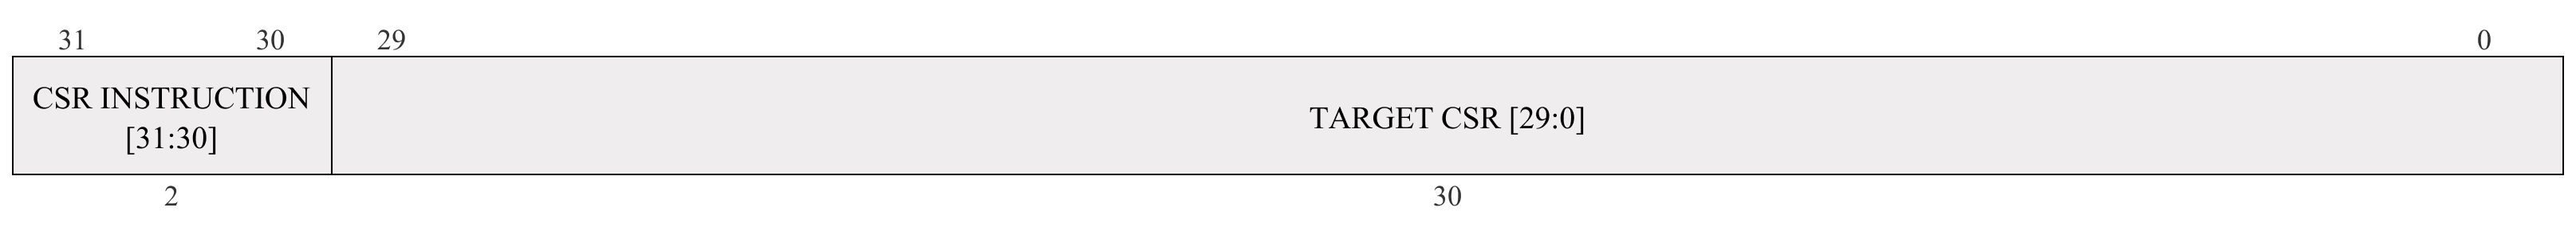
\includegraphics[width=.9\linewidth]{images/freertos_encoding.png}
  \caption{Possible encoding for register \textit{a6}}
  \label{fig:a6encoding}
\end{figure}

Inside the interrupt vector table, we would just need to add an if statement to
determine if we are requesting to perform a CSR instruction on behalf of \textit{FreeRTOS}
based on the \textit{ECALL} code. \\ \begin{lstlisting}[style=Assembly, caption = \textit{FreeRTOS} instrumentation for Control and Status Register operations, label={lst:csrinstrumentation}]
 mv a5, w_value      # Load the value to write into the CSR
 la a6, a6, csr      # Load the address of the target CSR
 ori a6, op_encoding # Load the encoding of the CSR operation
 addi a7, a7, ecode  # Load the new ECALL value
 ecall               # Perform the ECALL instruction
\end{lstlisting}

Note that this is just a proposal of implementation and there are other ways to
implement \textit{FreeRTOS} within the project. For example, instead of encoding
the CSR instruction inside register \textit{a6}, we could define an \textit{ECALL}
code for each operation and simply use that value to determine the operation to
perform. This would result in fewer instructions to instrument (as we could
remove the \textit{or} instruction) but would increase the size of the handler
as we would need to provide controls for each implemented \textit{ecode}.
